\documentclass[a4paper,10pt]{article}

\pagestyle{empty}


%%%%%%%%%%%%%%%%%%%%%%%%%%%%%%% Paquetes %%%%%%%%%%%%%%%%%%%%%%%%%%%%%%%%%%%

\usepackage[ansinew]{inputenc}
\usepackage[spanish]{babel}
\usepackage[mathcal]{euscript}
\usepackage{amsmath,amsfonts,amssymb,theorem,latexsym,mathrsfs, %hyperref,
            epsfig, multicol,anysize,graphicx,enumitem,mdwlist}
\usepackage{graphicx}  
\usepackage{ragged2e}  
\usepackage{float}        


%%%%%%%%%%%%%%%%%%%%%%%%%%%%%%%%%%%%%%%%%%%%%%%%%%%%%%%%%%%%%%%%%%%%%%%%%%%%


%%%%%%%%%%%%%%%%%%%%%%%%%%%%%%% M�rgenes %%%%%%%%%%%%%%%%%%%%%%%%%%%%%%%%%%%

\marginsize{2cm}{1.5cm}{1cm}{2cm}

%\marginsize{izquierdo}{derecho}{arriba}{abajo}

%%%%%%%%%%%%%%%%%%%%%%%%%%%%%%%%%%%%%%%%%%%%%%%%%%%%%%%%%%%%%%%%%%%%%%%%%%%%


%%%%%%%%%%%%%%%%%%%%%%%%%%%%% Definiciones %%%%%%%%%%%%%%%%%%%%%%%%%%%%%%%%%

\def\r{\mathbb{R}}
\def\n{\mathbb{N}}
\def\q{\mathbb{Q}}
\def\c{\mathbb{C}}
\def\z{\mathbb{Z}}

\def\sen{\mathop{\mbox{\normalfont sen}}\nolimits}
\def\intt{\mathop{\mbox{\normalfont int}}\nolimits}
\def\diag{\mathop{\mbox{\normalfont diag}}\nolimits}
\def\arcsen{\mathop{\mbox{\normalfont arcsen}}\nolimits}
\def\ln{\mathop{\mbox{\normalfont ln}}\nolimits}
\def\tr{\mathop{\mbox{\normalfont tr}}\nolimits}

%%%%%%%%%%%%%%%%%%%%%%%%%%%%%%%%%%%%%%%%%%%%%%%%%%%%%%%%%%%%%%%%%%%%%%%%%%%%

\begin{document}

%%%%%%%%%%%%%%%%%%%%%%%%%%%% Encabezado %%%%%%%%%%%%%%%%%%%%%%%%%%%%%%%%%%%%

\begin{minipage}{0.12\linewidth}

\includegraphics[width=15mm]{escudo.jpg}
\end{minipage}
\begin{minipage}{0.78\linewidth}
\centerline{UNIVERSIDAD DE ANTIOQUIA}
\centerline{Facultad de Ciencias Exactas y Naturales}
\centerline{Instituto de Matem�ticas}
\centerline{Series de Tiempo II}
\centerline{Taller $\#$ 3}
\end{minipage}

\vspace{3mm}

\leftline{Profesor: Duv�n Cata�o}


\vspace{8mm}


\begin{enumerate}

\item Muestre que un proceso ARFIMA$(0,d,0)$, con $-0,5<d<0,5$ tiene representaciones de la forma $z_t=\psi(B)a_t$ y $\pi(B)z_t=a_t$, con pesos dados por 
$$\psi_k=\frac{(k+d-1)!}{k!(d-1)!}, \ \ \ \ \ \ \  \pi_k=\frac{(k-d-1)!}{k!(-d-1)!},$$
respectivamente, donde $a_t\sim RB(0,\sigma_a^2).$ 

\bigskip

\item Demuestre que la densidad espectral de un proceso ARFIMA$(1,d,0)$ estacionario e invertible es dada por

$$f(w)=\frac{\sigma_a^2}{2\pi}\frac{[2\sin(0,5w)]^{-2d}}{(1+\phi^2-2\phi\cos w)}, \ \ \ 0<w\leq\pi,$$

adicionalmente que $$f(w)\approx\frac{\omega^{-2d}}{(1-\phi)^2},\ \ \ \ w\rightarrow0$$

\bigskip

%\item The data set $arf$ is 1000 simulated observations from an ARFIMA$(1, 1, 0)$ model with $\phi = 0.75$ and $d = 0.4.$
%\begin{enumerate}
%\item[a.] Plot the data and comment.
%\item[b.] Plot the ACF and PACF of the data and comment.
%\item[c.] Estimate the parameters and test for the significance of the estimates 
%$\hat{\phi}$ and $\hat{d}.$
%\item[d.] Explain why, using the results of parts (a) and (b), it would seem reasonable to difference the data prior to the analysis. That is, if $x_t$ represents the data, explain why we might choose to fit an ARMA model to $\nabla x_t.$
%\item[e.] Plot the ACF and PACF of $\nabla x_t$ and comment.
%\item[f.] Fit an ARMA model to $\nabla x_t$ and comment.
%\end{enumerate} 
\item Simular $T=1000$ observaciones $\{z_t\}$ de un proceso ARFIMA$(1,d,0)$, con $\phi=0,6$ y $d=0,45.$

\begin{enumerate}
    \item[a.] Haga un gr{\'a}fico de los datos simulados y comente.
    \item[b.] Calcule la ACF y PACF muestral y comente.
    \item[c.] Estime los par{\'a}metros del modelo, probando las significancia de cada            
    uno de ellos.
    \item[d.] Ajuste un modelo ARMA a $x_t=(1-B)z_t.$
    \item[e.] Compare el ajuste de los modelos ARFIMA ({\'i}tem c) y ARMA ({\'i}tem d).
\end{enumerate} 

\bigskip

%\item Compute the sample ACF of the absolute values of the NYSE returns displayed in Fig. 1.4 up to lag 200, and comment on whether the ACF indicates long memory. Fit an ARFIMA model to the absolute values and comment.

%\bigskip

\item Considere a serie $r_t$ de retornos diarios (cierre) del DJIA (archivo dow.xls). Sea la serie de retornos al cuadrado, $v_t = r_t^2$, que representa la 
serie de volatilidades.

  \begin{enumerate}
  \item[a.] Calcule las funciones de autocorrelaci{\'o}n y autocorrelaci{\'o}n parcial muestral   
  de la serie $v_t$ y comente.
  \item[b.] Identifique y estime un modelo de memoria larga para a serie $v_t$.
  \item[c.] Utilice el modelo final para hacer pron{\'o}stico con horizonte $l=6$. Haga  
  un gr{\'a}fico de la serie original y de los pron{\'o}sticos obtenidos.
  \end{enumerate}

\bigskip

\item Muestre que un modelo GARCH$(1,1)$ es equivalente a un modelo ARCH$(\infty)$, con pesos exponencialmente decrecientes.


\bigskip

\item Considere un modelo GARCH$(m,n)$. Calcular la media incondicional de los retornos al cuadrado. 

\bigskip

\item Weekly crude oil spot prices in dollars per barrel are in oil; see Problem Problem 2.10 and Appendix R for more details. Investigate whether the growth rate of the weekly oil price exhibits GARCH behavior. If so, fit an appropriate model to the growth rate.

\bigskip

\item The stats package of R contains the daily closing prices of four major European stock indices; type help(EuStockMarkets) for details. Fit a GARCH model to the returns of one of these series and discuss your findings. (Note: The data set contains actual values, and not returns. Hence, the data must be transformed prior to the model fitting.)











\end{enumerate}


\end{document}


% \begin{figure}[H]
%  \centering
%  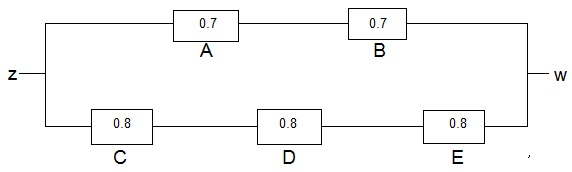
\includegraphics[width=.50\textwidth]{tab3}
% \end{figure}